In the figure (REF) the component interfaces belonging to the application server, with reference to what was shown in the Component diagram, are represented. The arrows represent a dependency relation.	
\begin{figure}[H]
    \centering
    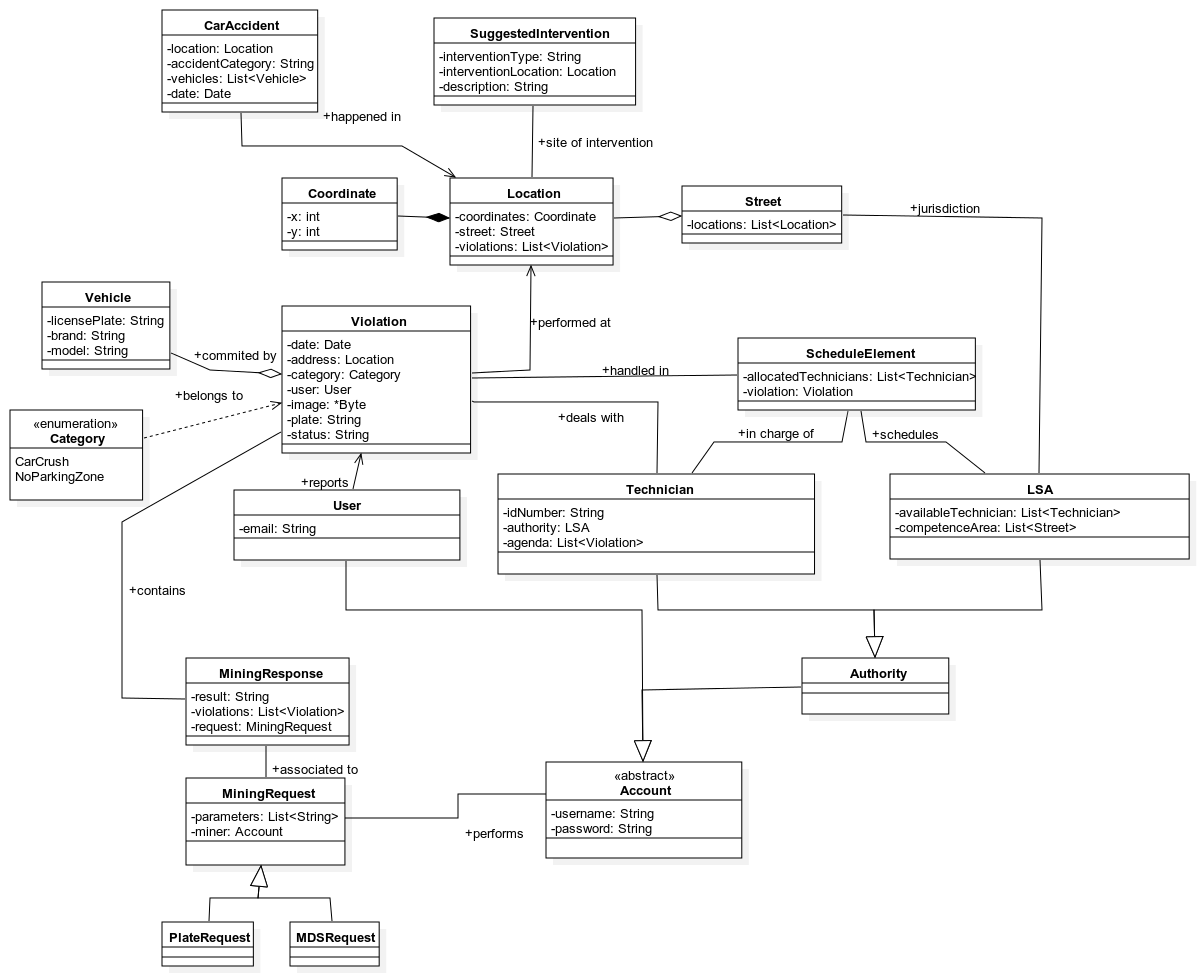
\includegraphics[width=1.1\textwidth]{UML_diagrams/class_diagram_safestreets}
    \caption{Class diagram}
    \label{fig:class_diagram}
\end{figure}
In figure \ref{fig:class_diagram}, the Safestreets class diagram is represented. This version of the class diagram is very similar to the one present in the RASD document, a part from:
\begin{itemize}
    \item The Mining request generalization, in order to add a new useful and extendible design pattern;
    \item The ScheduleElement class, which represents the n-n relation between Technicians and Violations: instead of representing this multiple relation in a singleton class which associate Technicians and Violations, the ScheduleElement objects represent tuples that links a single violation to many Technicians (<5 as stated in the RASD document). In this way, the system allows LSAs to schedule many Technicians to a specific violation as pictured in the web application mockups. The opposite operation (Technician to many violation) is not allowed up to this version of the system.
\end{itemize}